%!TEX root = ../../../2019main.tex
\vspace{10pt}
\subsubsection*{\bf Input and Output Optics}
\noindent {\sf [Spokesperson :\ Keiko KOKEYAMA]}

\vspace{3pt}
\noindent {\sf \small ICRR, The Univ.\ of Tokyo, Hida, Gifu 506-1205}

\vspace{3pt}

The input and output optics of KAGRA consists of the pre-stabilization system for the laser, auxiliary locking system, input optics chain, output optics chain. The pre-stabilization system includes the frequency stabilization system, intensity stabilization system, pre-mode cleaner, and modulation system for the main interferometer. The auxiliary locking system includes the phase locking system for the green beam each for X and Y arms, the fiber system, and the locking system for the arm cavities. The input optics chain includes the input mode cleaner, input Faraday isolator, and two input mode matching telescopes. The output optics chain includes the output mode matching telescopes, output Faraday isolator, and output mode cleaner. 

In the fiscal year of 2019, installations and commissioning works of most remaining systems have completed towards joining the O3 observation, as described below.

One of the major milestones in 2019 was the installation of the output optics chain. Three mirrors suspended by the type-C suspensions (double suspensions), output Faraday isolator, and output mode cleaner were installed. The three suspended mirrors are located downstream of the signal recycling mirror. The first two mirrors are the output mode matching telescopes (curved mirrors) and the third one is a steering mirror to steer the light to the output mode cleaner. The suspensions were developed by a collaboration with National Astronomical Observatory of Japan. The output Faraday isolator and output mode cleaner were developed and delivered from Tokyo Institute of Technology, and they were installed in the OMC chamber.
%OMC problem
After the installation of the output mode cleaner,
the finesse of the cavity was found to be around 300, much lower than the designed value of about 700.
By our investigations on an in-air optical bench,
one of the four mirrors of the output mode cleaner was found to be glued on the wrong side of the mirror wedge.
Due to the tilted mirror, the cavity eigenmode was off from the ideal beam axis,
and a beam spot on each mirror was off from its center.
Although the exact reason of the lower finesse was not clearly identified,
this can be one reason.
To fix the wrong eigenmode, the mirror was swapped with a spare one and glued at the right angle.
After changing the mirror, the measured finesse was confirmed as high as the design value in the air test bench.
However, the finesse measured in the vacuum chamber after the re-installation was 580.
The cause was not identified.
Fig. \ref{fig:omc} shows the photo of the output mode cleaner installed in the vacuum chamber.


\begin{figure}[t]
\begin{center}
\includegraphics[scale=0.15]{astrodiv/gw/ioo/omc.jpeg}
\caption{The output mode cleaner installed in the vacuum chamber.}
\label{fig:omc}
\end{center}
\end{figure}


For the input optics chain, by 2019, most of the important components had already installed and commissioned.
The target in 2019 was to improve the high power compatibility.
A beam shutter which can handle a high power beam was manufactured and installed in the pre-stabilized laser room.
The shutter is custom made based on one used in Advanced LIGO.
It is high-power compatible, and remotely controllable from the KAGRA control systems.
The shutter consists of a steering mirror attached on a solenoid which can rotate 45 degrees
so that the beam can be steered to the direction at 90 degrees to where a commercial high power beam dump
with a water cooling system is placed.
The installed shutter was found to fluctuate the beam
by heat caused at the shutter's solenoid,
as currents are applied on the solenoid when the shutter is open.
We temporarily circumvented the issue by swapping the solenoid to another one
whose rotation direction is opposite.
The solenoid's initial angle is also 45 degrees rotated compared with the original one
so that it opens when currents are not applied therefore when the solenoid is not heated.
However, from a safety point of view,
the shutter must close when the current is not applied.
The shutter has to be modified so in the near future.


The input mode cleaner which has been working since the iKAGRA phase
was tested with a high power for the first time.
The transmission power of 20 watts was achieved for about 50 minutes
without observing any thermal problems such as thermal lensing effects. 



A high power beam dump was specially designed, manufactured,
and installed in the IFI chamber with a team from National Astronomical Observatory of Japan.
It is to dump a high power beam, directly reflected light from the power recycling mirror (PRM), which is 90\% of the incident beam.
During initial alignment procedures and lock acquisition sequences,
the PRM is misaligned intentionally not to flash the power recycling cavity.
In such phases, the beam reflected by the misaligned PRM must be properly dump
not to damage any optics or suspension parts around it or not to significant scattered lights.
The beam dump must be vacuum compatible and to be able to
conduct the heat to outside of the vacuum enclosure.
The beam dump consists of a V-shape structure made from silicon carbide (SiC) plates.
The SiC plates are tightly fixed against copper holder parts with small Poly Ether Ether Ketonetes (PEEK) plates.
The upper half of the structure is made of also copper to have high thermal conductivity
whereas the lower half of the structure is a pedestal post made of SUS
which as a smaller thermal conductivity compared with copper
so not to heat up the optical table under the pedestal.
Ten copper heat sinks are used to release the heat to the outside of the flange.
The sinks are bolted the copper part on one side,
and the other side is linked to the vacuum flange of an OFC (oxygen-free-copper) disk
of 230 mm in diameter and 20 mm thick,
so that a heat is conducted and released to the atmosphere.
A platinum thermal probe is attached on the top of the V-shape part
so that the temperature of the beam dump can be monitored.
The overall picture is depicted in Fig. \ref{fig:dump}
By the high power test of the input mode cleaner mentioned in the previous paragraph,
the heat flow of the dump was also tested.
As a result, we found that the heat flow needs to be modified.
The temperature of the dump did not raise as expected,
which suggests the majority of the heat was conducted by the SUS pedestal to the table.
\begin{figure}[t]
\begin{center}
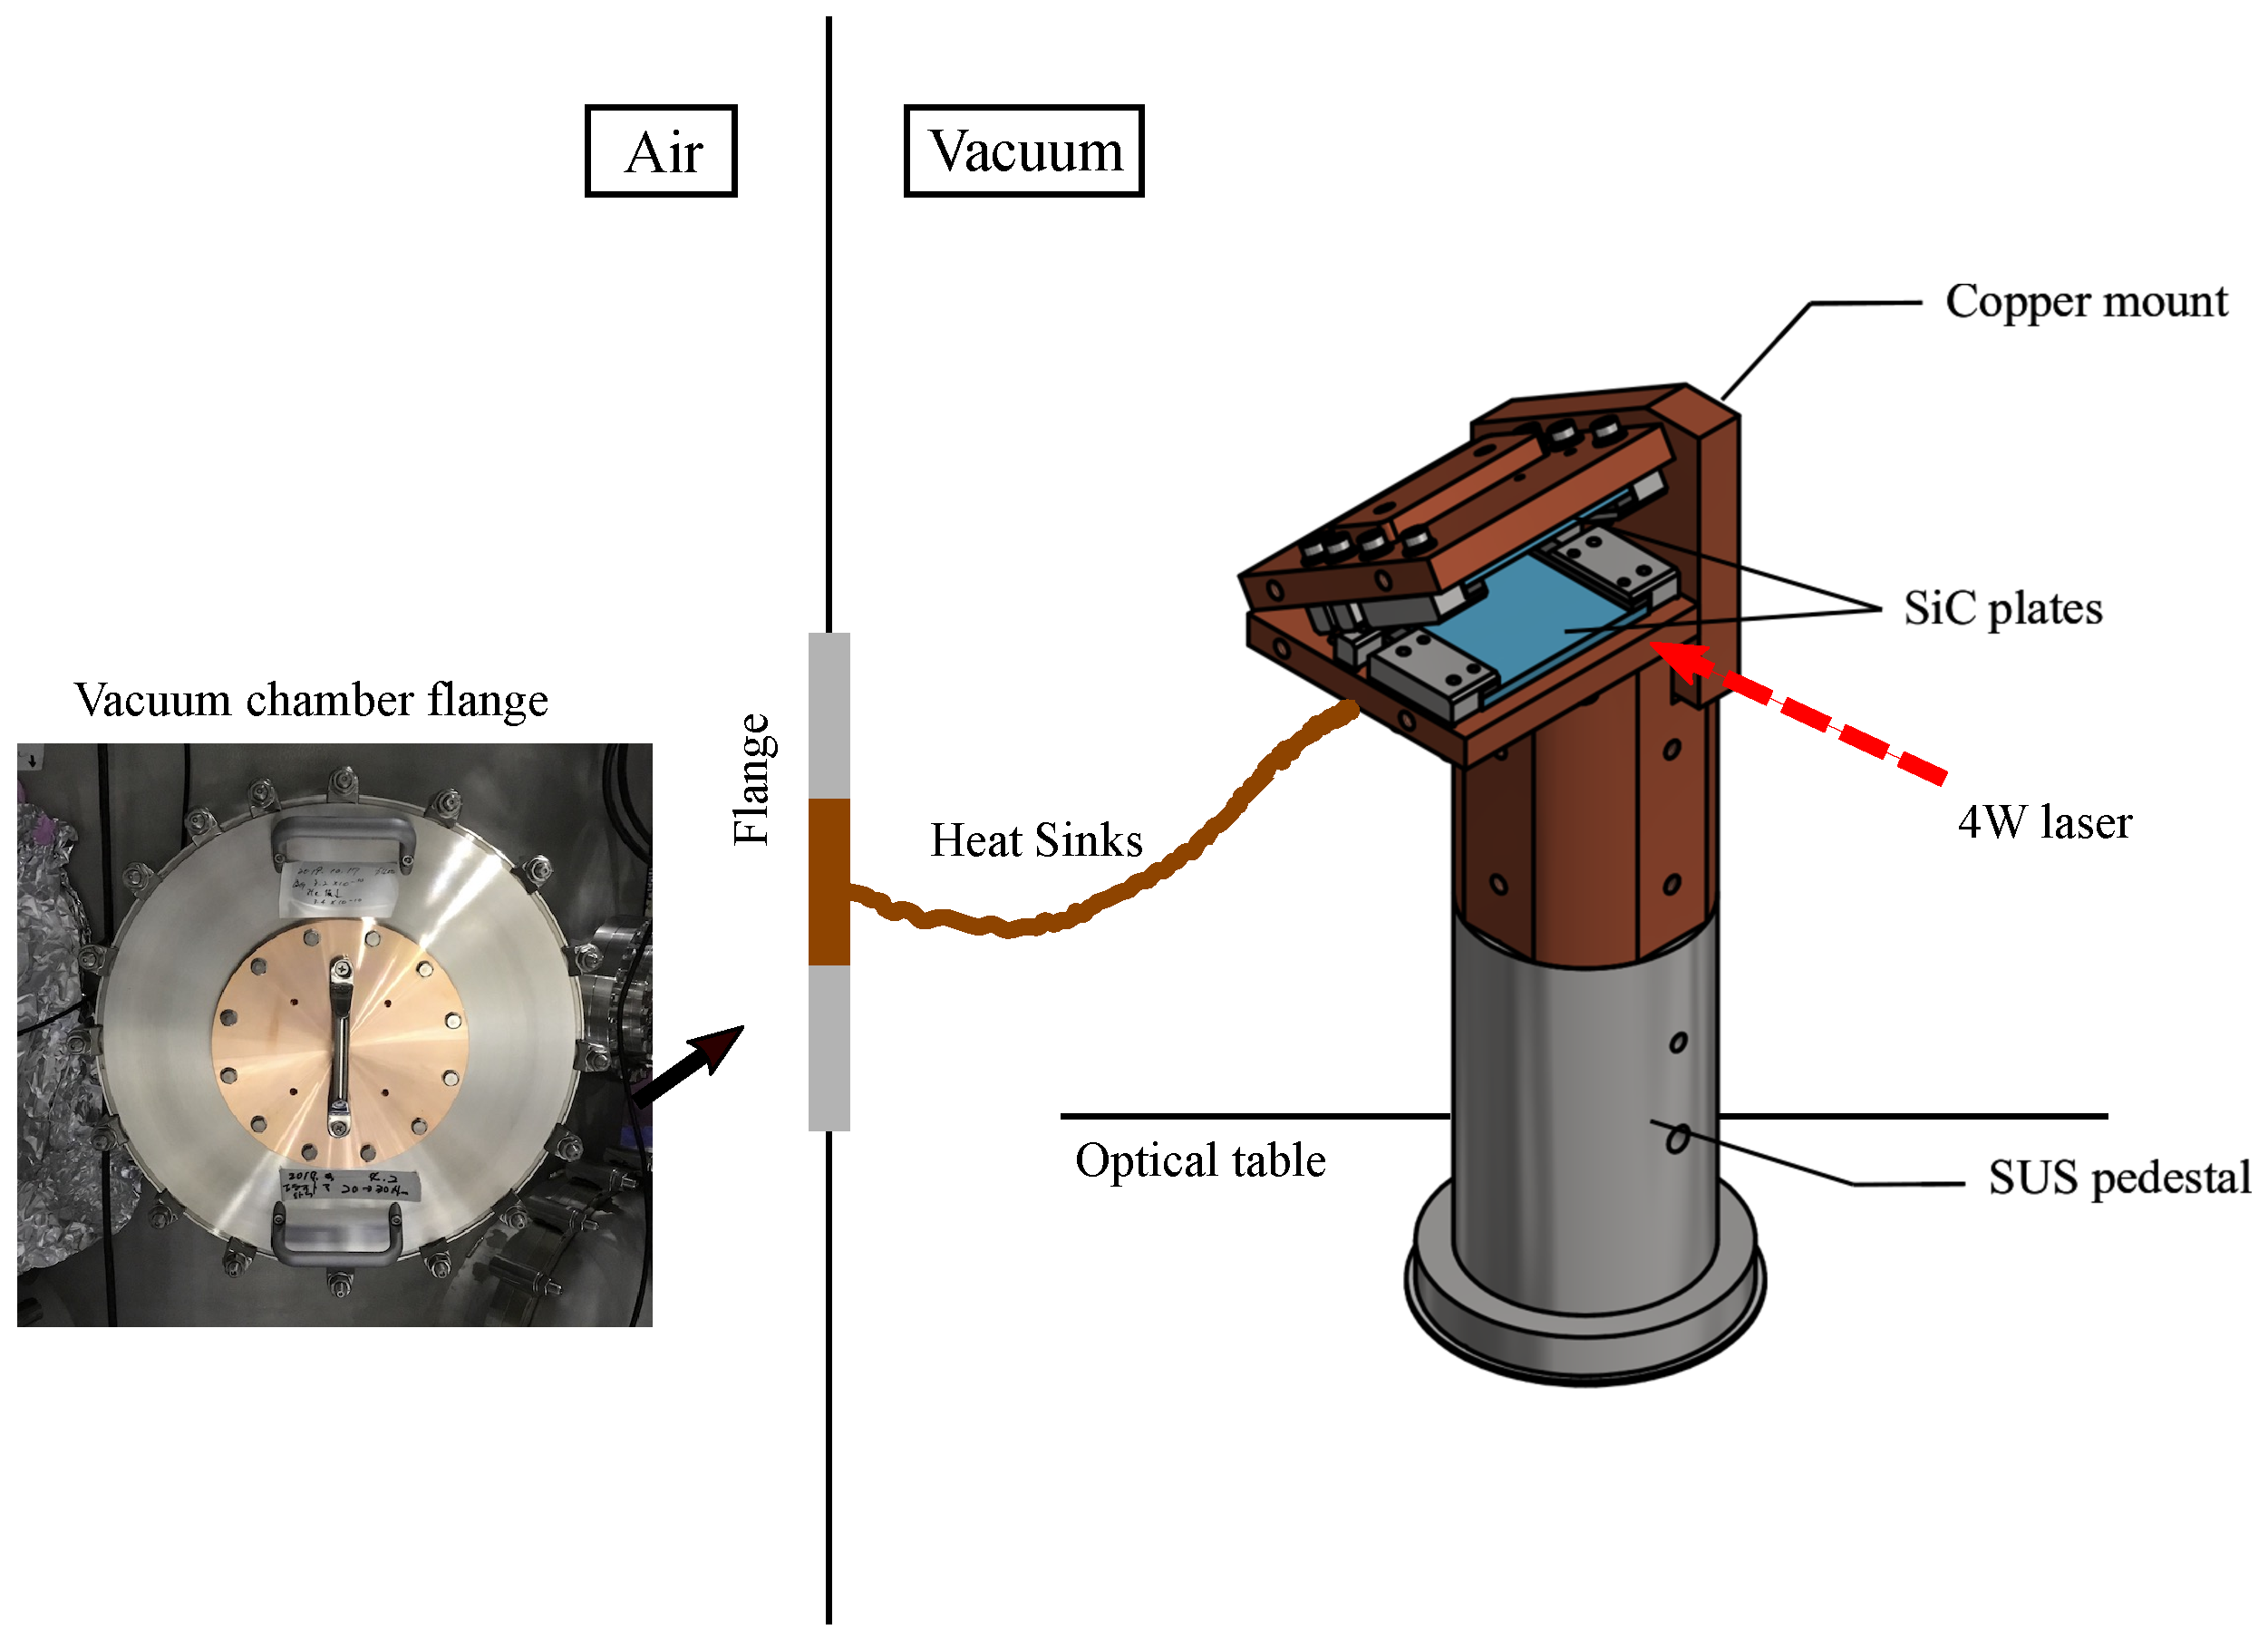
\includegraphics[scale=0.2]{astrodiv/gw/ioo/dump_figure2.eps}
\caption{The overall picture of the high power beam dump
including the heat conduction path.}
\label{fig:dump}
\end{center}
\end{figure}



In addition to the development of the high power beam dump,
to protect the suspension fibers from exposures by the high power beam,
solblack coated (light absorbing material by Asahi precision Co. Ltd.) metal plates
were attached on the type-C suspensions of input mode-matching telescopes
in the IFI and IMM chambers, as shown in Fig. \ref{fig:shield}.

\begin{figure}[t]
\begin{center}
\includegraphics[scale=0.15]{astrodiv/gw/ioo/shield.jpeg}
\caption{Solblack coated shields were installed on input mode-matching telescopes
to protect from direct exposures of high power laser beam.}
\label{fig:shield}
\end{center}
\end{figure}


In parallel of the experiments mentioned above, a proof-of-principle experiment
for the Mach-Zehnder Modulation system (MZM) was successfully conducted.
In the final phase of the KAGRA operation, aiming the quantum noise demolition, 
the signal recycling cavity will be detuned to produce optical springs.
At the detuning phase, the signal recycling cavity is known to introduce great excess noise,
a new modulation scheme to relax the noise coupling was proposed \cite{ioo:dt}.
The new modulation system is with two Mach-Zehnder interferometer in series (MZM),
and can apply both phase and amplitude modulations at an arbitrary ratio between them,
by applying a phase difference between the oscillator signals on the corresponding two electro-optic modulators.
Our proof-of-principle experiment successfully verified the new feature
of variable ratio between the phase and amplitude modulations.
It was done as a topic of a master thesis of an ICRR student.
The result was published in \cite{ioo:mzm}.

%\bibitem{ioo:dt} S. Ueda, K Somiya et al., Class. Quantum Grav. 31 095003 (2014)
%\bibitem{ioo:mzm} K Yamamoto et al., Class. Quantum Grav. 36 (2019) 205009.


